\chapter{Practical application of DFT}
\label{sec:Practical DFT}

In this section we will present the practical application and implementation of density functional theory in the study of materials science.

\section{The Exchange-Correlation functional}
\textbf{Add references and other fixes later}

From the former section, we know that the only peace of information we require to perform DFT plane-wave calculations are that of the exchange-correlation energy $E_{\text{xc}}[n]$. Given that the functional properties of a material is strongly related to the electronic density, the precision of DFT is very sensitive to the type of approximation to the density. The initial challenge is to balance the factors affecting the accuracy of the model to the computational cost.

The exchange-correlation functional is only exactly known for a homogeneous electron gas, however this is of limited use in real materials with variation in the electron concentration. An improvement on this is the local density approximation (LDA), in which the electronic density is set at each position according to the homogeneous electron gas at that position, in other words
\begin{equation}
    V_{xc}(\vec{r}) = V_{xc}^{\text{e gas}}[n(\vec{r})]
\end{equation}
This is seen as a successful approximation for the exchange-correlation energy in bulk materials, given that typically the electron density does not vary tremendously. However this method is not without flaws, most notably is the presence/degree of self-interaction from the fact that this term does not completely cancel out by only including the local environment. This may lead to artificial contributions to $V_{xc}$ and an overall inaccurately high electron density. The success behind this method most reliably lies in the low computational cost. 

The generalized gradient approximation (GGA) extends on the concept of LDA by also including the gradient of the electron density. 
\begin{equation}
    V_{xc}^{GGA}(\vec{r}) = V_{xc}[n(\vec{r}), \nabla n(\vec{r})].
\end{equation}
GGA is good for materials with a slowly varying density, but fails with large gradients. The GGA functional is implemented in two different methods, Perdew-Wang 91 (PW91) and Perdew-Burke-Ernzerhof (PBE). This method can further be extended to include the second order gradient, methods with this approach are called meta-GGA. Popular implementations include \textit{Modified Becke and Johnson} (MBJ) and \textit{Strongly Constrained Appropriately Normed} (SCAN). \textbf{write SCAN later}

Both methods underestimate the band gap and wrongly predict the charge localization in cases of narrow bands or lattice distortion. A large part of this comes from the self-interaction of the Hartee potential. By combining the correlations and exchange of LDA/GGA with the exact exchange of the Hartree-Fock approximation, we can obtain much more precise calculations. This method was proposed by Becke as hybrid functionals, since the functional is a hybrid between the two. This method is superior in describing localized states, but comes at a significant larger computational cost. In order to reduce this cost, Heyd al et. split the Hartree-Fock exchange into short-range and long-range parts, in which calculations can adapt exact Hartree-Fock exchange for short-range (SL) and non-exact for long-range (LR). By introducing the parameter $\omega$ to adjust the order parameter of the method, we can express this method, called HSE (Heyd-Scuseria-Ernzerhof) as
\begin{equation}
    E_{xc}^{HSE} = \alpha E_{x}^{HF,SR}(\omega) + (1-\alpha)E_{x}^{PBE, SR}(\omega) + E_x^{PBE,LR}(\omega) + E_{c}^{PBE}
\end{equation}
\begin{itemize}
    \item Explain what the different notations mean, and the success + limitations of HSE compared to LDA and GGA.
    \item Write a paragraph on meta-GGA, such as SCAN and perhaps MBJ.
\end{itemize}

\section{Fundamental aspects of practical DFT calculations}
With the exchange-correlation functionals presented above, we now have everything in order to perform DFT calculations. To begin solving eq .., we need the single-electron wave-function, for a free electron this is a plane wave $\psi_k = Ae^{i\boldsymbol{k}\boldsymbol{r}}$. In a solid however, there exist a nonzero periodic potential $V(\boldsymbol{r}) = V(\boldsymbol{r} + \boldsymbol{R})$, the solution to the Shr\"{o}dinger equation is given by Bloch's theorem wich states that the solution takes the form
\begin{equation}
\psi_{\boldsymbol{k}}(\boldsymbol{r}) = u_{\boldsymbol{k}}(\boldsymbol{r})e^{i\boldsymbol{k}\boldsymbol{r}},    
\end{equation}
where $u_{\boldsymbol{k}}(\boldsymbol{r}$ is a bloch wave with identical periodicity to the supercell. And $\boldsymbol{k}$ is the wavevector. Along with eq(above), problems in DFT are solved in k-space or reciprocal space for convience sake. For instance a great deal of DFT calculations revolve around solving the integral 
\begin{equation}
    g = \frac{V_{\text{cell}}}{(2\pi)^3} \int_{\text{BZ}} g(\boldsymbol{k})d\boldsymbol{k},
\end{equation}
with BZ denoting that the integral be evaluated for all $\boldsymbol{k}$ in the Brillouin zone. This integral can be approximated by evaluating the integral at a set of discrete points and summing over the points with appropriatly assigined weigts. A larger set of points leads to more exact approximations. This method is called Legendre quadrature. The method for selceting these points in reciprocal space was devolped by Monkhorst and Pack in 1976, and simply put requieres a amount of kpoints in each direction in reciprocal space, in the form $N x N x N$. Recalling that reciprocal space is inverse to regular space, supercells with equal and large dimensions converge at smaller values of N, and inversly for cells of small dimsion. In supercells with different length axis, such as hexagonal cells, we use the notation $N x N x M$, where $M$ relate to the distincntly different axis. The amount of kpoints required can be fruther reduced by utulizing the symmetry of the cell, in which we can exactly approximate the entire BZ by extending a lesser zone through symmertry. This reduced zone is appropriartly named the irreducible Brillouin zone (IBZ). 

Metals in particular requiere a large set of kpoints to acchive accurate results. This is becouse we encounter discontinuies functions in the Brillouin zone around the fermi sufrace where the states discontinusly change from occupied to non-occupied. To reduce the cost of this operatin, there are two primary methods, tetrhaedon and smearing. The idea behind the tetrahedon method is to use the discrete set of k-points to fill the reciprocal space with tethraeda and interpolate the function within each tethraeda such that the function can be integrated in the entire space rather than at discrete points. The latter approach for solving discontinuos integrals is to smear out the discontinuity and thus transforming the integral to a continous one. A good analogy to this method is the fermi-dirac function, in which a small variable $\sigma$ transform a step-functino into a continious function that can be integrated by standard methods.

In addition to the number of kpoints, there is one more distinct parameter that must be specified in DFT calculations, namely the energy cutoff, or $E_{\text{cut}}$. This parameters arise from the Bloch function described previosly. In which $u_{\boldsymbol{k}}(\boldsymbol{r})$ was a bloch wave with the same periodicity as the supercell. This implies that the wave can be expanded by a set of special plane waves as
\begin{equation}
    u_{\boldsymbol{k}}(\boldsymbol{r}) = \sum_{\boldsymbol{G}} c_{\boldsymbol{G}}e^{i\boldsymbol{G}\boldsymbol{r}},
\end{equation}
where $\boldsymbol{G}$ is the reciprocal lattice vector. Combining this with eq ..(first eq for blcoh function) we get 
\begin{equation}
    \psi_{\boldsymbol{k}}(\boldsymbol{r}) = \sum_{\boldsymbol{G}} c_{\boldsymbol{k} + \boldsymbol{G}}e^{i(\boldsymbol{k} + \boldsymbol{G})\boldsymbol{r}}
\end{equation}
The consequense from this expression is that evaluating the wavefunction of an electron at a single $k$ point demand a summation over the entirity of reciprocal space. In order to reduce this computational burden, we can introduce a maximum paramater $E_{\text{cut}}$ to cap the calculations. This is possible becouse eq ..(above) is the solution of the Shr\"{o}dinger equation with kinetic energy 
\begin{equation}
    E = \frac{\hbar^2}{2m}|\boldsymbol{k} + \boldsymbol{G}|^2.
\end{equation}
Seeing as the solution with lower energies are the most interesting, we can limit the calculations of eq ..(2 above) to solutions with energy less than $E_{\text{cut}}$ given bellow
\begin{equation}
    E_{\text{cut}} = \frac{\hbar^2}{2m}G_{\text{cut}}.
\end{equation}
Thus, we can reduce the infinitly large sum above to a much more feasable calculation in 
\begin{equation}
    \psi_{\boldsymbol{k}}(\boldsymbol{r}) = \sum_{|\boldsymbol{k} + \boldsymbol{G}| < G_{\text{cut}}} c_{\boldsymbol{k} + \boldsymbol{G}}e^{i(\boldsymbol{k} + \boldsymbol{G})\boldsymbol{r}}
\end{equation}

\textbf{A summary on kpoints and ENCUT, plus a discussion on nummerical convergence and how to select kpoints and ENCUT}


A final consideration to how DFT is applied in practise is how the core electrons are handled. Tightly bound core electrons as opposed to valene electrons demand a greater number of plane-waves to converge. The most efficient method of reducing the expenses of core-electrons are so-called pseudopotentials. This method works by approximating the electron density of the core elecrons by a constant density that mimic the properties of true ion core and core electrons. This density is then remained constant for all subsequent calculations, ie only considering the valence electrons while regarding the core electrons as frozen-in. There are currently two popular types of psudopotentials used in DFT, so-called ultrasoft psudopotentials (USPPs) devoplped by Vanderbilt, and the projecter augmented-wave (PAW) method by Bloch. This project will exclusivly apply the latter. 

\section{Self-consistent calculation}

\begin{figure}
\centering
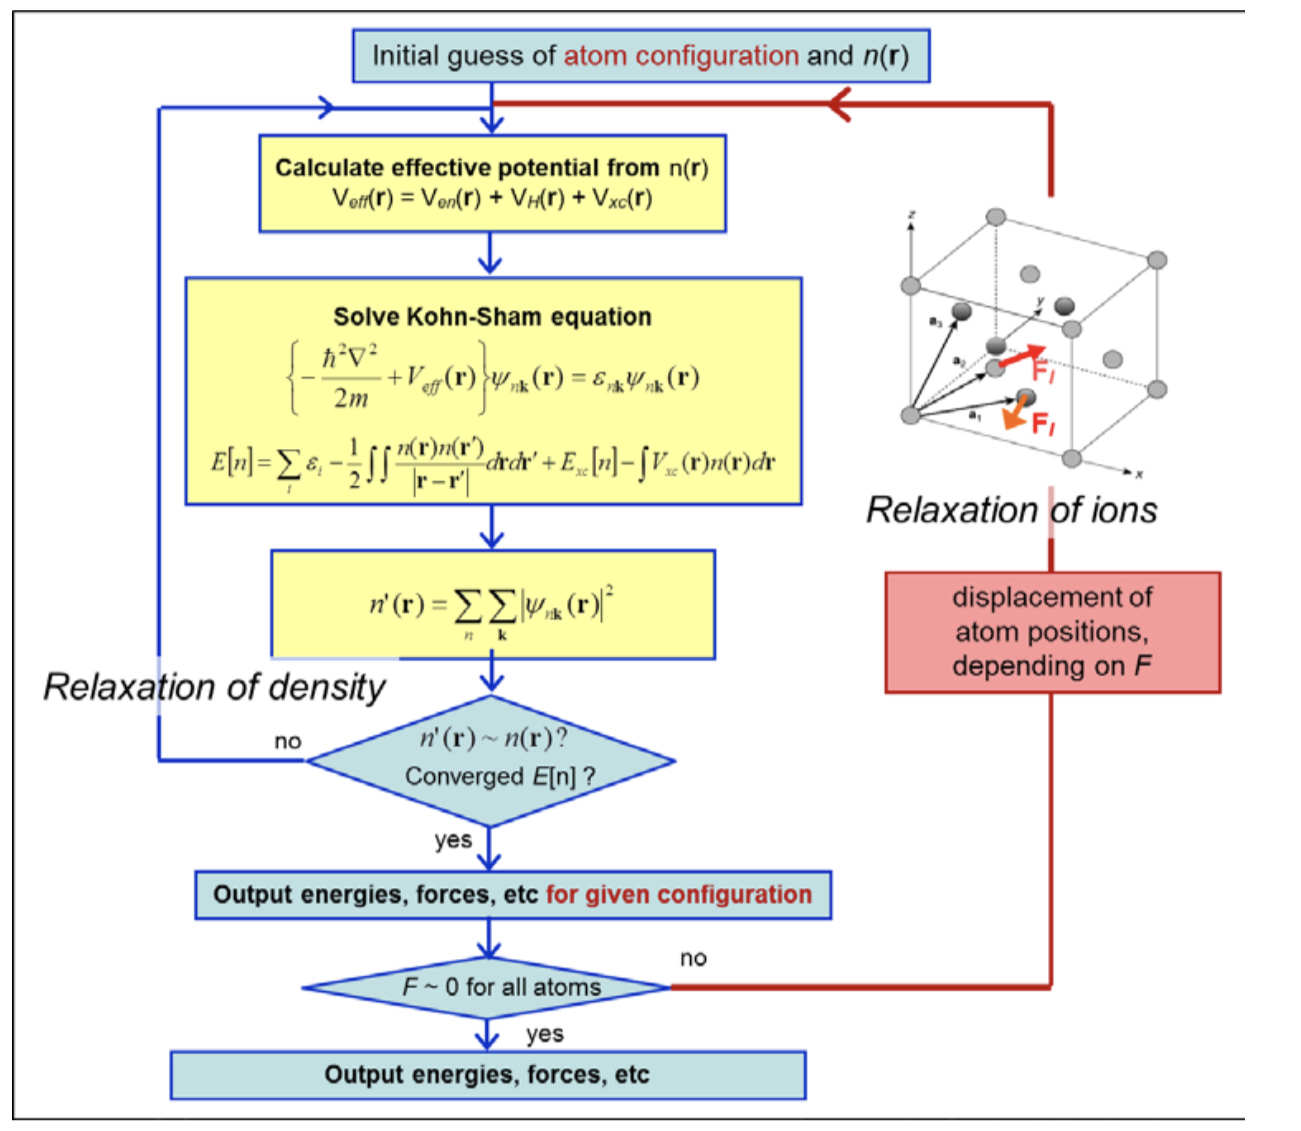
\includegraphics[scale=.3]{theory/selfConsistentDFT.jpeg}
\caption{Self consistent iteration of a DFT calculation. Figure adopted from ..}
\label{sfDFT}
\end{figure}